\documentclass[12pt]{article}


\usepackage{setspace}
\usepackage{indentfirst}
\usepackage {array}
\usepackage {booktabs}


\usepackage {enumitem}
\usepackage {pgfplots}
\usepackage {circuitikz}
\usepackage {caption}

\begin{document}

\begin{center}
    \textbf{\large ABSTRACT}
\end{center}

Man has needed and used energy at an increasing rate for the sustenance and well-being since time immemorial. Due to this, a lot of energy resources have been exhausted and wasted. Proposal for the utilization of waste energy of foot power with human locomotion is very much relevant and important for highly populated countries like India where the railway station, temples etc., are overcrowded all round the clock. When the flooring is engineered with piezo electric technology, the electrical energy produced by the pressure is captured by floor sensors and converted to an electrical charge by piezo transducers, then stored and used as a power source. And this power source has many applications as in agriculture, home application and street lighting and as energy source for sensors in remote locations.

This paper is all about generating electricity when people walk on the floor. Think about the forces you exert which is wasted when a person walks. The idea is to convert the weight energy to electrical energy. The power generating floor intends to translate the kinetic energy to the electrical power. Energy Crisis is the main issue of the world these days. The motto of this research work is to face this crisis somehow. Though it won’t meet the requirement of electricity but as a matter of fact if we are able to design a power generating floor that can produce 100W on just 12 steps, then for 120 steps we can produce 1000W and if we install such type of 100 floors with this system then it can produce 1MegaWatt. Which itself is an achievement to make it significant.

\vspace{1cm}

\begin{flushright}
    \textbf{JIEMS, Akkalkuwa}
\end{flushright}

   \newpage



\section*{List of Figures}
\begin{table}[h!]
\centering
\begin{tabular}{|c|p{8cm}|c|}
\hline
\textbf{Sr. No} & \textbf{Figure} & \textbf{Page No.} \\ \hline
1 & Model of Foot Step Energy Generation & 05 \\ \hline
2 & Block Diagram & 06 \\ \hline
3 & Schematic Representation of the Working Model & 08 \\ \hline
4 & Connection Diagram & 15 \\ \hline
5 & Sample and Hold Circuit & 19 \\ \hline
6 & Power Generation Pie Chart & 20 \\ \hline
\end{tabular}
\end{table}

\vspace{1cm}

\section*{List of Symbols and Abbreviations}
\begin{table}[h!]
\centering
\begin{tabular}{|c|p{10cm}|}
\hline
\textbf{Sr. No} & \textbf{Abbreviations} \\ \hline
1 & GaPO4 (Gallium Phosphate) \\ \hline
2 & CAD (Computer Aided Design) \\ \hline
3 & RL (Load Resistance) \\ \hline
4 & FSEC (Foot Step Electric Converter) \\ \hline
5 & ADC (Alternating to Direct Current Converter) \\ \hline
\end{tabular}
\end{table}

\vspace{1cm}

\begin{flushright}
    \textbf{JIEMS, Akkalkuwa}
\end{flushright}


\newpage



\newpage 


\section*{Contents}
\begin{table}[h!]
\centering
\begin{tabular}{|c|p{9cm}|c|}
\hline
\textbf{Sr. No} & \textbf{Topic} & \textbf{Page No.} \\ \hline
1  & Introduction & 04 \\ \hline
2  & Model of Footstep Energy Generation & 05 \\ \hline
3  & Block Diagram \& Working & 06 \\ \hline
4  & Energy Storing Table & 07,08 \\ \hline
5  & Need of That System & 08 \\ \hline
6  & Maximum Theoretical Voltage Generated & 09 \\ \hline
7  & Analysis Done on the Piezo Tile & 10,11 \\ \hline
8  & Sensor \newline $\bullet$ Piezoelectric Sensor & 11,12,13 \\ \hline
9  & Battery Connection \newline $\bullet$ Series \& Parallel & 13,14,15 \\ \hline
10 & Unidirectional Current Controller \newline $\bullet$ Diode \newline $\bullet$ Thyristors & 17 \\ \hline
11 & Voltage Sampler (Sample \& Hold Circuit) & 18,19,20 \\ \hline
12 & Advantage and Disadvantage & 21 \\ \hline
13 & Application & 22 \\ \hline
14 & Conclusion & 23 \\ \hline
15 & Reference & 24 \\ \hline
\end{tabular}
\end{table}

\vspace{1cm}

\begin{flushright}
    \textbf{JIEMS, Akkalkuwa}
\end{flushright}

\newpage 

\section*{Introduction}

For an alternate method to generate electricity, there are a number of methods by which electricity can be produced. Out of such methods, footstep energy generation can be an effective method to generate electricity.

Walking is the most common activity in human life. When a person walks, he loses energy to the road surface in the form of impact, vibration, sound, etc., due to the transfer of his weight to the road surface, through footfalls on the ground during every step. This energy can be tapped and converted into a usable form such as in electrical form. This device, if embedded in the footpath, can convert foot impact energy into electrical form.

Human-powered transport has been in existence since time immemorial in the form of walking, running, and swimming. However, modern technology has led to machines to enhance the use of human power in a more efficient manner. In this context, pedal power is an excellent source of energy and has been in use since the nineteenth century, making use of the most powerful muscles in the body. Ninety-five percent of the exertion put into pedal power is converted into energy. Pedal power can be applied to a wide range of jobs and is a simple, cheap, and convenient source of energy. However, human kinetic energy can be useful in a number of ways, but it can also be used to generate electricity based on different approaches, and many organizations are already implementing human-powered technologies to generate electricity to power small electronic appliances.

 \newpage 



\section*{Model of Footstep Energy Generation}

\begin{figure}[h!]
    \centering
    \includegraphics[width=0.7\textwidth]{footstep_device.jpg} % Replace with actual image file name
    \caption{Storing Device for Footstep Electric Energy}
\end{figure}

The working of the Foot Step Electric Converter (FSEC) is demonstrated in photographs. The right-side photograph shows the foot touching the top plate without applying weight. The left-side photograph shows the foot when the full weight of the body is transferred to the top plate. A 6 W, 12 V bulb connected to the output of the alternator glows to indicate the electric output when foot load is applied. The unit is designed to generate a full power pulse when actuated by a person weighing nearly 60 kg. An experimental plot of voltage vs. time was generated using an oscilloscope. Using voltage data and the load (a resistor), a typical plot of power vs. time was generated.

The power generated by the footstep generator can be stored in an energy-storing device. The output of the generator was fed to a 12 V lead-acid battery through an AC-DC converter bridge. Initially, the battery was completely discharged. Then, the FSEC was operated by applying foot load, and energy was stored in the battery. A 100 W, 230 V bulb was connected to the battery through an inverter. The arrangement is shown in Fig. 4. The duration of lighting the bulb for a number of footsteps and the corresponding energy stored are given in Table 1.

 \newpage 

\section*{Block Diagram}

\begin{figure}[h!]
    \centering
    \includegraphics[width=0.8\textwidth]{block_diagram.jpg} % Replace with actual image file name
    \caption{Block Diagram of the Footstep Energy Generation System}
\end{figure}

\section*{Working Principle}

\begin{itemize}[leftmargin=1.5cm]
    \item The basic working principle of our project is based on the piezoelectric sensor.
    \item To implement this, we adjust the wooden plates above and below the sensors and movable springs.
    \item Non-conventional energy using footsteps converts mechanical energy into electrical energy.
    \item The footstep board consists of 16 piezoelectric sensors connected in parallel.
    \item When pressure is applied to the sensors, they convert mechanical energy into electrical energy.
    \item This electrical energy is stored in a 12V rechargeable battery connected to an inverter.
    \item A conventional battery charging unit is also used to supply the circuitry.
    \item The inverter converts the 12V DC into 230V AC, which activates the loads.
    \item Using this AC voltage, we can operate AC loads.
\end{itemize}

\newpage

\section*{Energy Storing Table}

The power generated by the footstep generator can be stored in an energy storing device. The output of the generator was fed to a 12 V lead-acid battery, through an AC-DC converter bridge. Initially, the battery was completely discharged. Then, the FSEC was operated by applying foot load and energy was stored in the battery. A 100 W, 230 V bulb was connected to the battery through an inverter. The arrangement is shown in Fig. 4. The duration of lighting, the bulb for the number of footsteps and corresponding energy stored, are given in Table~1.

\begin{table}[h!]
\centering
\begin{tabular}{cccc}
\toprule
\textbf{No. of Footsteps} & \textbf{Duration of lighting a} & \textbf{Total Energy (J)} & \textbf{Energy/Step (J)} \\
                          & \textbf{100 W 230 V Bulb (s)}   &                            &                           \\
\midrule
250                       & 6                               & 600                        & 2.4                       \\
500                       & 12                              & 1,200                      & 2.4                       \\
750                       & 18                              & 1,800                      & 2.4                       \\
1,000                     & 25                              & 2,500                      & 2.5                       \\
\bottomrule
\end{tabular}
\caption{Energy stored per number of footsteps.}
\end{table}

The piezoelectric material converts the pressure applied to it into electrical energy. The source of pressure can be either from the weight of the moving vehicles or from the weight of the people walking over it. The output of the piezoelectric material is not a steady one. So a bridge circuit is used to convert this variable voltage into a linear one. Again, an AC ripple filter is used to filter out any further fluctuations in the output. The output DC voltage is then stored in a rechargeable battery.

As the power output from a single piezo-film was extremely low, a combination of a few Piezo films was investigated. Two possible connections were tested—parallel and series connections. The parallel connection did not show a significant increase in the voltage output. With series connection, additional piezo-film results in increased voltage output but not in linear proportion. So here a combination of both parallel and series connections is employed for producing 40 V DC output with high current density. 

From the battery, provisions are provided to connect the load. An inverter is connected to the battery to provide a provision to connect AC load. The voltage produced across the tile can be seen in an LCD.


\newpage


\section*{Fig: Schematic Representation of the Working Model}

\begin{center}
\includegraphics[width=0.8\textwidth]{schematic_placeholder} % Replace 'schematic_placeholder' with the filename of the actual image
\end{center}

\section*{Need of That System}

\begin{itemize}[leftmargin=1.5cm]
    \item Proposal for the utilization of waste energy of foot power with human locomotion is very much relevant and important for highly populated countries like India and China where the roads, railway stations, bus stands, temples, etc., are all overcrowded and millions of people move around the clock. This whole human/bioenergy being wasted, if made possible for utilization, will be a great invention, and crowd energy farms will be very useful energy sources in crowded countries. Walking across a ``Crowd Farm'' floor will be fun for idle people who can improve their health by exercising in such farms with earning. The electrical energy generated at such farms will be useful for nearby applications.
    
    \item The utilization of waste energy of foot power with human motion is very important for highly populated countries.
    
    \item India and China, where the roads, railway stations, temples, etc., are all overcrowded, and millions of people move around the clock.
\end{itemize}


\newpage

\section*{Maximum Theoretical Voltage Generated}

When a force is applied on piezo material, a charge is generated across it. Thus, it can be assumed to be an ideal capacitor. Therefore, all equations governing capacitors can be applied to it. In this project, on one tile, we connect 3 piezoelectric discs in series. Ten such series connections are connected in parallel. Thus, when 3 piezoelectric discs are connected in series, their equivalent capacitance becomes:

$$ \frac{1}{C_{\text{eq}}} = \frac{1}{C_1} + \frac{1}{C_2} + \frac{1}{C_3} $$

We know,
$$ Q = C \cdot V $$

So,
$$ C = \frac{Q}{V} $$

Hence,
$$ \frac{V_{\text{eq}}}{Q} = \frac{V_1}{Q} + \frac{V_2}{Q} + \frac{V_3}{Q} $$

Thus,
$$ V_{\text{eq}} = V_1 + V_2 + V_3 $$

Hence, the net voltage generated in a series connection is the sum of individual voltages generated across each piezoelectric disc. The output voltage from one piezoelectric disc is 13V.

Thus,
$$ V_{\text{eq}} = V_1 + V_2 + V_3 $$
$$ = 13 + 13 + 13 $$
$$ = 39 \, \text{V} $$

Thus, the maximum voltage that can be generated across the piezo tile is around 39V.

 \newpage 


\begin{figure}[h!]
\centering
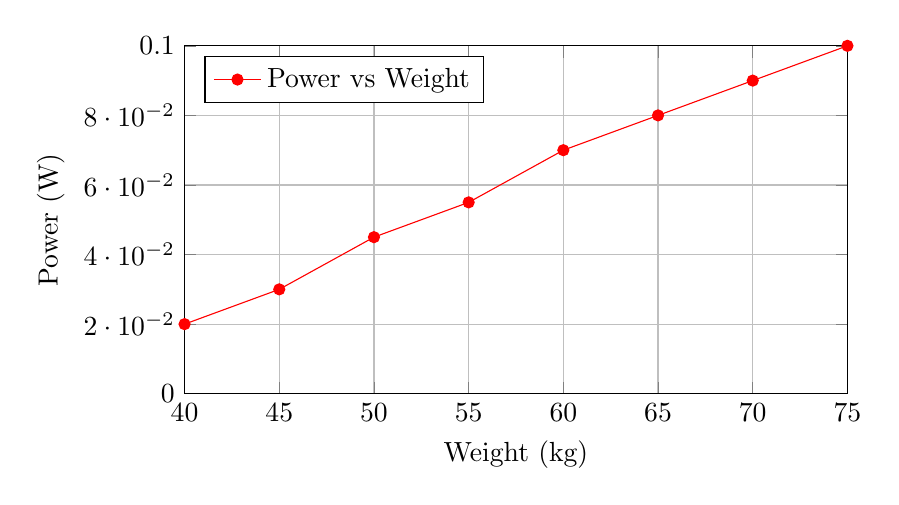
\begin{tikzpicture}
    \begin{axis}[
        xlabel={Weight (kg)},
        ylabel={Power (W)},
        xmin=40, xmax=75,
        ymin=0, ymax=0.1,
        xtick={40,45,50,55,60,65,70,75},
        ytick={0,0.02,0.04,0.06,0.08,0.1},
        legend pos=north west,
        grid=major,
        width=10cm, height=6cm
    ]
        \addplot[color=red,mark=*] coordinates {
            (40, 0.02)
            (45, 0.03)
            (50, 0.045)
            (55, 0.055)
            (60, 0.07)
            (65, 0.08)
            (70, 0.09)
            (75, 0.1)
        };
        \addlegendentry{Power vs Weight}
    \end{axis}
\end{tikzpicture}
\caption{Weight V/s Power graph of piezo tile}
\label{fig:piezo_tile_graph}
\end{figure}



\newpage

\section*{Human Locomotion and Energy Conversion}
Human locomotion in overcrowded subway stations, railway stations, bus stands, airports, temples, or rock concerts can thus be converted to electrical energy with the use of this promising technology.

The technology would turn the mechanical energy of people walking or jumping into a source of electricity. The students' test case, displayed at the Venice Biennale and in a train station in Torino, Italy, was a prototype stool that exploits the passive act of sitting to generate power. The weight of the body on the seat causes a flywheel to spin, which powers a dynamo that, in turn, lights four LEDs. In each case, there would be a sub-flooring system consisting of independent blocks. When people walk across this surface, the forces they impart will cause the blocks to slip slightly, and a dynamo would convert the energy in those movements into electric current. Students say that moving from this proof-of-concept device to a large-scale Crowd Farm would be expensive, but it certainly sounds a great option.

\section*{Sensor}
A sensor is a device that measures a physical quantity and converts it into a signal which can be read by an observer or by an instrument. For example, mercury converts the measured temperature into expansion and contraction of a liquid which can be read on a calibrated glass tube. A thermocouple converts temperature to an output voltage which can be read by a voltmeter. For accuracy, most sensors are calibrated against known standards.

\subsection*{Piezoelectric Sensor}
A piezoelectric sensor is a device that uses the piezoelectric effect to measure pressure, acceleration, strain, or force by converting them into an electrical signal. Piezoelectric sensors have proven to be versatile tools for the measurement of various processes. They are used for quality assurance, process control, and for research and development in many different industries. It was only in the 1950s that the piezoelectric effect started to be used for industrial sensing applications.

\newpage



Since then, this measuring principle has been increasingly used and can be regarded as a mature technology with an outstanding inherent reliability. It has been successfully used in various applications, such as in medical, aerospace, nuclear instrumentation, and as a pressure sensor in the touch pads of mobile phones. In the automotive industry, piezoelectric elements are used to monitor combustion when developing internal combustion engines. The sensors are either directly mounted into additional holes into the cylinder head, or the spark/glow plug is equipped with a built-in miniature piezoelectric sensor.

\begin{center}
    \includegraphics[width=0.6\textwidth]{piezoelectric_sensor_placeholder} % Replace "piezoelectric_sensor_placeholder" with the file name of the image
\end{center}

\begin{center}
    \textbf{Fig: Piezoelectric Sensor}
\end{center}

The rise of piezoelectric technology is directly related to a set of inherent advantages. The high modulus of elasticity of many piezoelectric materials is comparable to that of many metals and goes up to \( 10^6 \, \text{N/m}^2 \). Even though piezoelectric sensors are electromechanical systems that react to compression, the sensing elements show almost zero deflection. This is the reason why piezoelectric sensors are so rugged, have an extremely high natural frequency, and an excellent linearity over a wide amplitude range. 

Additionally, piezoelectric technology is insensitive to electromagnetic fields and radiation, enabling measurements under harsh conditions. Some materials used (especially gallium phosphate or tourmaline) have an extreme stability even at high temperatures, enabling sensors to have a working range of up to \( 1000^\circ \text{C} \). Tourmaline shows piezoelectricity in addition to the piezoelectric effect; this is the ability to generate an electrical signal when the temperature of the crystal changes. This effect is also common to piezoceramic materials.

\newpage

One disadvantage of piezoelectric sensors is that they cannot be used for truly static measurements. A static force will result in a fixed amount of charges on the piezoelectric material. While working with conventional readout electronics, imperfect insulating materials, and reduction in internal sensor resistance will result in a constant loss of electrons, and yield a decreasing signal.

\includegraphics[width=0.5\textwidth]{diagram_placeholder} % Replace "diagram_placeholder" with the file name of the diagram

Elevated temperatures cause an additional drop in internal resistance and sensitivity. The main effect on the piezoelectric effect is that with increasing pressure loads and temperature, the sensitivity is reduced due to twin-formation. While quartz sensors need to be cooled during measurements at temperatures above 300$^\circ$C, special types of crystals like GaPO4 gallium phosphate do not show any twin formation up to the melting point of the material.

\section*{Battery}

Battery (electricity), an array of electrochemical cells for electricity storage, either individually linked or individually linked and housed in a single unit. An electrical battery is a combination of one or more electrochemical cells, used to convert stored chemical energy into electrical energy.
\newpage 


Batteries may be used once and discarded, or recharged for years as in standby power applications. Miniature cells are used to power devices such as hearing aids and wristwatches; larger batteries provide standby power for telephone exchanges or computer data centers.

\begin{center}
    \includegraphics[width=0.6\textwidth]{battery_image_placeholder} % Replace "battery_image_placeholder" with the actual file name of the image
\end{center}

\begin{center}
    \textbf{Fig: Battery}
\end{center}

Lead-acid batteries are the most common in PV systems because their initial cost is lower and because they are readily available nearly everywhere in the world. There are many different sizes and designs of lead-acid batteries, but the most important designation is that they are deep cycle batteries. Lead-acid batteries are available in both wet-cell (requires maintenance) and sealed no-maintenance versions. Lead-acid batteries are reliable and cost-effective with an exceptionally long life. The Lead-acid batteries have high reliability because of their ability to withstand overcharge, over-discharge, vibration, and shock.

The use of special sealing techniques ensures that our batteries are leak-proof and non-spoilable. The batteries have exceptional charge acceptance, large electrolyte volume, and low self-discharge, which make them ideal as zero-maintenance batteries. Lead-acid batteries are manufactured/tested using CAD (Computer-Aided Design). These batteries are used in Inverter \& UPS Systems and have the proven ability to perform under extreme conditions. The batteries have electrolyte volume, use PE Separators, and are sealed in sturdy containers, which give them excellent protection against leakage and corrosion.


\newpage


\section*{Battery Connections}

Lead-acid batteries are normally available in blocks of 2V, 6V, or 12V. In most cases, to generate the necessary operating voltage and the capacity of the batteries for the Solar Inverter, many batteries have to be connected together in parallel and/or in series. Following three examples are shown:

\subsection*{Series Connection}
\begin{center}
    \includegraphics[width=0.8\textwidth]{series_connection_placeholder} % Replace "series_connection_placeholder" with the file name of the series connection diagram
\end{center}
\begin{center}
    \textbf{Fig: Series Connection (12V)}
\end{center}

\subsection*{Parallel Connection}
\begin{center}
    \includegraphics[width=0.8\textwidth]{parallel_connection_placeholder} % Replace "parallel_connection_placeholder" with the file name of the parallel connection diagram
\end{center}
\begin{center}
    \textbf{Fig: Parallel Connection (12V)}
\end{center}

\newpage 
\section*{Rectifier}
The output from the transformer is fed to the rectifier. It converts A.C. into pulsating D.C. The rectifier may be a half-wave or a full-wave rectifier. In this project, a bridge rectifier is used because of its merits like good stability and full-wave rectification. 

The bridge rectifier is a circuit that converts an AC voltage to DC voltage using both half cycles of the input AC voltage. The bridge rectifier circuit is shown in the figure. The circuit has four diodes connected to form a bridge. The AC input voltage is applied to the diagonally opposite ends of the bridge. The load resistance is connected between the other two ends of the bridge.

For the positive half cycle of the input AC voltage, diodes D1 and D3 conduct, whereas diodes D2 and D4 remain in the OFF state. The conducting diodes will be in series with the load resistance $R_L$ and hence the load current flows through $R_L$. For the negative half cycle of the input AC voltage, diodes D2 and D4 conduct, whereas D1 and D3 remain OFF.

The conducting diodes D2 and D4 will be in series with the load resistance $R_L$ and hence the current flows through $R_L$ in the same direction as in the previous half cycle. Thus, a bi-directional wave is converted into a unidirectional wave.

\section*{Voltage Regulator}
As the name itself implies, it regulates the input applied to it. A voltage regulator is an electrical regulator designed to automatically maintain a constant voltage level. In this project, power supplies of 5V and 12V are required. 

In order to obtain these voltage levels, 7805 and 7812 voltage regulators are to be used. The first number 78 represents positive supply, and the numbers 05 and 12 represent the required output voltage levels. These regulators can provide local on-card regulation, eliminating the distribution problems associated with single-point regulation. Each type employs internal current limiting, thermal shutdown, and safe area protection, making it essentially indestructible.
\newpage
\section*{Unidirectional Current Controller}

As the name indicates, this circuit allows only one direction current flowing. There are the following devices that allow unidirectional current:

\begin{enumerate}
    \item Diode
    \item Thyristors
\end{enumerate}

In this project, we are going to use a diode as a Unidirectional Current control device. As we are already familiar, the most common function of a diode is to allow an electric current to pass in one direction (called the diode's forward direction) while blocking current in the opposite direction (the reverse direction). Thus, the diode can be thought of as an electronic version of a check valve. The diode used in this project is \(D = \text{1N4007}\).

\section*{ADC (A/D or A to D)}

An analog-to-digital converter (abbreviated ADC, A/D, or A to D) is a device that converts a continuous quantity to a discrete time digital representation. An ADC may also provide an isolated measurement. The reverse operation is performed by a digital-to-analog converter (DAC).

Typically, an ADC is an electronic device that converts an input analog voltage or current to a digital number proportional to the magnitude of the voltage or current. However, some non-electronic or only partially electronic devices, such as rotary encoders, can also be considered ADCs.
\newpage
\section*{Inverter}

An inverter is an electrical device that converts direct current (DC) to alternating current (AC); the converted AC can be at any required voltage and frequency with the use of appropriate transformers, switching, and control circuits.

Solid-state inverters have no moving parts and are used in a wide range of applications, from small switching power supplies in computers, to large electric utility high-voltage direct current applications that transport bulk power. Inverters are commonly used to supply AC power from DC sources such as solar panels or batteries.

There are two main types of inverter. The output of a modified sine wave inverter is similar to a square wave output except that the output goes to zero volts for a time before switching positive or negative. It is simple and low cost and is compatible with most electronic devices, except for sensitive or specialized equipment, for example certain laser printers.

A pure sine wave inverter produces a nearly perfect sine wave output ($<3\%$ total harmonic distortion) that is essentially the same as utility-supplied grid power. Thus it is compatible with all AC electronic devices. This is the type used in grid-tie inverters.

Its design is more complex, and costs 5 or 10 times more per unit power. The electrical inverter is a high-power electronic oscillator. It is so named because early mechanical AC to DC converters was made to work in reverse, and thus were ``inverted'', to convert DC to AC. The inverter performs the opposite function of a rectifier.

\section*{Voltage Sampler (Sample \& Hold Circuit)}

Sample-and-hold (S/H) is an important analog building block with many applications, including analog-to-digital converters (ADCs) and switched-capacitor filters. The function of the S/H circuit is to sample an analog input signal and hold this value over a certain length of time for subsequent processing.
\newpage 
 \begin{circuitikz}
    % Input voltage
    \draw (0,0) node[anchor=east] {$V_{in}$} to[short] (1,0);

    % First op-amp
    \draw (1,0) to[R, l_=33k] (3,0) -- (3,2)
        to[empty diode, l=1N4148] (5,2) -- (5,0)
        to[short, *-] (6,0) node[op amp, anchor=+](opamp1){412};

    % MOSFET and hold capacitor
    \draw (3,0) to[generic, l=MPF102] (3,-2)
        to[C, l=0.1] (5,-2) -- (5,0);
    \draw (3,-2) -- (1,-2) to[R, l=1M] (1,0);

    % Output voltage
    \draw (opamp1.-) -- ++(0,-1) node[ground] {};
    \draw (opamp1.out) -- ++(2,0) node[anchor=west] {$V_{out}$};

    % Voltage sources
    \draw (3,-2) node[anchor=east] {-12} to[short] ++(0,-0.5)
        node[ground] {};

    % Label
    \node at (3,-3) {Sample-and-Hold Circuit};
\end{circuitikz}


Taking advantages of the excellent properties of MOS capacitors and switches, traditional switched capacitor techniques can be used to realize different S/H circuits. The simplest S/H circuit in MOS technology is shown in Figure, where Vin is the input signal, MI is an MOS transistor operating as the sampling switch, Ch is the hold capacitor, ck is the clock signal, and Vout is the resulting sample-and-hold output signal.

In the simplest sense, a S/H circuit can be achieved using only one MOS transistor and one capacitor. The operation of this circuit is very straightforward. Whenever ck is high, the MOS switch is on, which in turn allows Vout to track Vin. On the other hand, when ck is low, the MOS switch is off.

During this time, Ch will keep Vout equal to the value of Vin at the instance when ek goes low. CMOS Sample-and-Hold Circuits Page Unfortunately, in reality, the performance of this S/H circuit is not as ideal as described above. The next section of this paper explains two major types of errors, charge injection.

and clock feed through, that are associated with this S/H implementation. The section after that presents three new S/H techniques, all of which try to minimize the errors caused by charge injection and/or clock feed through..

\newpage
\section*{Power Generation Analysis}

As we know, the pressure is directly proportional to the amount of power generated:
\[
P \propto Wt
\]
Here we take the constant of proportionality as \(K\), then the equation becomes:
$$ P = K \cdot Wt $$
Where,  
\begin{itemize}
    \item \(K\) - Constant of proportionality
    \item \(Wt\) - Weight
    \item \(P\) - Power
\end{itemize}

We know that for \(Wt = 50\, \text{kg}\), we get the value of voltage \(V = 4\, \text{V}\) and current \(I = 0.015\, \text{A}\).  
Then:
$$ P = V \cdot I = 4 \cdot 0.015 = 0.06\, \text{W} $$
This means we can say that for \(50\, \text{kg}\), we get power:
$$ P = 0.06\, \text{W} $$
From this, we can find the value of \(K\):
$$ K = \frac{P}{Wt} = \frac{0.06}{50} = 0.0012 $$

\section*{Power Generation Pie Chart}

\begin{figure}[h!]
    \centering
    \includegraphics[width=0.8\textwidth]{pie_chart_placeholder.png} % Replace with the actual file name of the pie chart image
    \caption{Power generation in India}
    \label{fig:pie_chart}
\end{figure}
\newpage 
\section*{Foot-Step Power Generator}

\subsection*{Advantages}
\begin{itemize}[noitemsep]
    \item Power generation is simply walking on a step.
    \item No need for fuel input.
    \item This is a non-conventional system.
    \item No moving parts - long service life.
    \item Self-generating - no external power required.
    \item Compact yet highly sensitive.
    \item Reliable, economical, eco-friendly.
    \item Less consumption of non-renewable energies.
    \item Power also generated by running or exercising on the step.
    \item Battery is used to store the generated power.
    \item Extremely wide dynamic range, almost free of noise.
\end{itemize}

\subsection*{Disadvantages}
\begin{itemize}[noitemsep]
    \item Only applicable for a particular place.
    \item Initial cost of this arrangement is high.
    \item Output affected by temperature variation.
    \item Care should be taken for batteries.
\end{itemize}
\newpage
\section*{Foot-Step Power Generator}

\subsection*{Application}
\begin{itemize}[noitemsep]
    \item Foot-step generated power can be used for agricultural, home applications, street lighting.
    \item Foot-step power generation can be used in emergency power failure situations.
    \item Metros, rural applications, etc.
    \item It can be used as a source for both A.C. and D.C. applications.
    \item It is also used in universities.
    \item It can be used in emergency power failure situations like hospitals.
\end{itemize} 
\newpage
\section*{Foot-Step Power Generator}

\subsection*{Conclusion}
\begin{enumerate}[noitemsep]
    \item The project \textbf{``Power Generation Using Foot Step''} is successfully tested and implemented, which is the best economical, affordable energy solution to common people.
    \item This can be used for many applications in rural areas where power availability is less or totally absent. As India is a developing country where energy management is a big challenge for a huge population, using this project, we can drive both A.C. as well as D.C. loads according to the force applied on the piezoelectric sensor.
\end{enumerate}

A piezo tile capable of generating 40V has been devised. Comparison between various piezoelectric materials shows that PZT is superior in characteristics. Also, by comparison, it was found that series-parallel combination connection is more suitable. The weight applied on the tile and corresponding voltage generated is studied, and they are found to have a linear relation. It is especially suited for implementation in crowded areas. This can be used in street lighting without the use of long power lines. It can also be used as charging ports and lighting of pavement side buildings.

As a fact, only 11\% of renewable energy contributes to our primary energy. If this project is deployed, then not only can we overcome the energy crisis problem, but this also contributes to creating a healthy global environmental change.

\begin{itemize}[noitemsep]
    \item Smart system.
    \item Produces 2000 watts of electricity.
    \item Durable.
    \item Has a life of approx. 5 years.
\end{itemize}
\newpage
\begin{thebibliography}{99}

\bibitem{fakhzan2013}  
M.N. Fakhzan, G.A. Muthalif, "Vibration Based Energy Harvesting Using Piezoelectric Material," Department of Mechatronics Engineering, International Islamic University Malaysia, IIUM, Kuala Lumpur, Malaysia.

\bibitem{piezoelectric2013}  
"Piezoelectric Crystals: Future Source Of Electricity," International Journal of Scientific Engineering and Technology, Volume 2, Issue 4, April 2013, Third Year.

\bibitem{footsteps2004}  
S.S. Talyian, B.B. Biswas, R.K. Patil, G.P. Srivastava, and T.K. Basu, "Electricity from Footsteps," Reactor Control Division, Electronics & Instrumentation Group, IPR, Gandhinagar.

\bibitem{strain2004}  
Henry A. Sodano, Daniel J. Inman, Gyuhae Park, "Estimation of Electric Charge Output for Piezoelectric Energy Harvesting," LA-UR-04-2449, Strain Journal, 40(2), 49-58, 2004.

\bibitem{virginia2010}  
"Center for Intelligent Material Systems and Structures," Virginia Polytechnic Institute and State University.

\bibitem{zhu2010}  
Meiling Zhu, Emma Worthington, Ashutosh Tiwari, "Design Study of Piezoelectric Energy-Harvesting Devices for Generation of Higher Electrical Power Using a Coupled Piezoelectric-Circuit Finite Element Method," IEEE Transactions on Ultrasonics, Ferroelectrics, and Frequency Control, vol. 57, no. 2, February 2010.

\end{thebibliography}

\end{document}